% \documentclass[10pt, conference, compsocconf]{IEEEtran}
%\documentclass[conference]{IEEEtran}
\documentclass{sig-alternate}
\usepackage{eso-pic,xcolor}
\makeatletter
%
\pdfpagewidth=8.5in
\pdfpageheight=11in
\usepackage{flushend}
%\AddToShipoutPicture*{%
%\setlength{\@tempdimb}{20pt}%
%\setlength{\@tempdimc}{\paperheight}%
%\setlength{\unitlength}{1pt}%
%\put(\strip@pt\@tempdimb,\strip@pt\@tempdimc){%
%   \makebox(0,-60)[l]{\color{blue}%
%
%  }%
  
%\put(\strip@pt\@tempdimb,\strip@pt\@tempdimc){%
%    \makebox(0,-85)[l]{\color{black}%
%}%
%}%

%\put(\strip@pt\@tempdimb,\strip@pt\@tempdimc){%
%    \makebox(0,-110)[l]{\color{black}%
%}%
%  }%
%}

%
\def\ps@headings{%
\def\@oddhead{\mbox{}\scriptsize\rightmark \hfil \thepage}%
\def\@evenhead{\scriptsize\thepage \hfil \leftmark\mbox{}}%
\def\@oddfoot{}%
\def\@evenfoot{}}
\makeatother




\pagestyle{headings}

\title{NDNlive and NDNtube: Live and Pre-recorded \\\ Video Streaming over NDN}

\author{
%Paper \#231, 13 pages
Lijing Wang \\ {\normalsize Tsinghua University} \\ {\normalsize wanglj11@mails.tsinghua.edu.cn }
\and Ilya Moiseenko \\ {\normalsize UCLA} \\ {\normalsize iliamo@cs.ucla.edu }
\and Lixia Zhang \\ {\normalsize UCLA} \\ {\normalsize lixia@cs.ucla.edu }
}


\newfont{\nicettfont}{cmtt10}
\newcommand{\ndnName}[1]{``{\nicettfont #1}''}
\renewcommand{\texttt}[1]{{\nicettfont #1}}

\newcommand{\todo}[1]{\vspace{2 mm}\par \noindent \marginpar{\textsc{ToDo}}
\framebox{\begin{minipage}[c]{0.95 \columnwidth}
\tt #1 \end{minipage}}\vspace{5 mm}\par}

\usepackage{graphicx}
% \usepackage[colorlinks]{hyperref}
\usepackage[]{hyperref}
%\usepackage{breakurl}
\usepackage{url}
\usepackage[nocompress]{cite}
\usepackage{amsmath}
% \usepackage{verbatim}
% \usepackage{algpseudocode}
\usepackage{algpseudocode,algorithm}
% More customizeable version. Probably it would be better to convert pseudocode to 2e format
% \usepackage{algorithm2e} 
\usepackage{multirow}
\usepackage{times}
\usepackage{color}
\paperheight=11in
\graphicspath{{figures/}}

\begin{document}

\maketitle

\begin{abstract}
Named Data Networking offers significant promise for content distribution applications, such as video playback application. Two NDN-based video projects are proposed in this technical report: NDNLive and NDNTube. They are live and pre-recorded video streaming project over NDN, which follows the ADU(Application Data Unit) designing pattern. Video and Audio stream are chopped into individual frames and get published and retrieved by Consumer / Producer API. NDNLive and NDNTube have shown some basic usages of this API. By naming every frame individually provides the flexibility and efficiency to application implementation.
\end{abstract}


%\begin{IEEEkeywords}
%Information-centric networks, named data networking, API, inter-process communication
%\end{IEEEkeywords}
\input{01introduction}
%!TEX root = nextndnvideo-tr.tex
\section{background} % (fold)
\label{sec:background}
\subsection{Consumer / Producer API}
Consumer-Producer API~\cite{api-tr} provides a generic programming interface to NDN communication protocols and architectural modules. A consumer context associates an NDN name prefix with various data fetching, transmission, and content verification parameters, and integrates processing of Interest and Data packets on the consumer side. A producer context associates an NDN name prefix with various packet framing, caching, content-based security, and namespace registration parameters, and integrates processing of Interest and Data packets on the producer side.

In NDNlive and NDNtube, the video publisher consists of multiple producers generating video and audio frames separately. The corresponding video players consist of multiple consumers sending Interests for the video and audio frames. Consumer / Producer API simplifies the application logic at both sides: media production and media consumption. Since video frames are too large to be encapsulated by a single Data packet, the media production pipeline has to include a content segmentation step in order to split the content into multiple Data packets. Producer API provides this segmentation functionality. At the same time, since a video frame cannot be retrieved by a single Interest packet, UDR and RDR protocols behind the Consumer API automatically pipeline Interest packets and solve other tasks related to the retrieval of the application frame. 
%In the case of MPEG-DASH, all these low-level details are handled by the HTTP / TCP protocol machinery. 
We will talk about the implementation details in Section~\ref{sec:implementation}.

\subsection{Gstreamer}

We use Gstreamer~\cite{gstreamer} to handle the media processing part. 

In NDNLive, raw video images captured by the camera are transferred to the \textit{Encoder\_v} component and are encoded into \textit{H264} format. Then the encoded video is passed to the \textit{Parser\_v} to be parsed into frames (\textit{B, P or I frame}). The microphone captures the raw audio, which is passed to the \textit{Encoder\_a}. The encoder component encodes the raw audio into \textit{AAC} format. The encoded audio stream is transferred to the \textit{Parser\_a} to be parsed into audio frames, which are passed to the Producer API for any possible segmentation. Video and audio data is retrieved frame by frame that are passed to the video \textit{Decoder\_v} and audio \textit{Decoder\_a} for the decoding into the format which the video \textit{Player\_v} or audio \textit{Player\_a} can play.

In NDNTube, the source for video and audio streams is an mp4 file containing \textit{H264} video and \textit{AAC} audio. Gstreamer opens the file and passes it to the \textit{Demuxer} component to separate video and audio streams. Since the video file is already encoded, the media processing pipeline does not have an \textit{Encoder} component in it. The encoded video or audio streams are separately pushed into the \textit{Parser} to generate video and audio frames.

%Because we need to extract the frames from the video source, so now we only support \textit{H264} video encoded format and  encoded format for NDNLive and \textit{MP4} file format for NDNTube. 

\subsection{Repo-ng}
NDNLive streams the captured video and audio non-stop. Therefore, the media publisher just keeps producing new frames and does not care about the data it produced several minutes ago. The consumer is also interested only in recent video and audio frames. As long as the producer is attached to the NDN network, it  will serve the incoming Interests. %The consumer can get the data back and play them back immediately.

NDNTube publishes the video only once --- all Data packets corresponding to audio and video frames are permanent and never change after the initial publication. Since the same video could be requested multiple times by different users, it is reasonable to store the produced Data packets in a `database' which is exposed to the requests from the network. Otherwise, every time a different user requests the same video, the corresponding video and audio Data packets would have to be republished (and signed) in case NDN cache has not been able to satisfy these Interests.

Repo-ng~\cite{repo-ng} is used as a permanent storage for the video and audio content. Repo-ng (repo-new generation) is an implementation of NDN persistent in-network storage, which exposes a Repo protocol~\cite{Repo-Protocol} allowing write access to applications. Repo insertion is natively supported by the Producer API with \textit{LOCAL\_REPO} option (if repo is running on the local host) or \textit{REMOTE\_REPO\_PREFIX} option to point to the right remote repo by its name prefix. 
% section section_name (end)
%!TEX root = nextndnvideo-tr.tex
\vspace{0.3cm}
\section{design goals} % (fold)
\label{sec:design_goals}

% section section_name (end)
%!TEX root = nextndnvideo-tr.tex
\vspace{0.3cm}
\section{Design} % (fold)
\label{sec:arch}
NDNlive and NDNtube are composed of two roles: publisher and player. Both publisher and player make use of appropriate parts of Consumer / Producer API to simplify the design of the system.

\paragraph{NDNlive architecture} % (fold)
\vspace{0.3cm}
\label{par:ndnlive_arch}
Figure~\ref{fig:ndnlive_arch} illustrates the architecture of NDNLive, which can be summarized as follows:

\begin{itemize}
  \item \textit{Publisher}

  NDNlive is a \textit{live streaming} application, therefore the publisher captures video from camera and audio from microphone, and passes it to the Gstreamer to get raw data encoded and extracted as video and audio frames. The video and audio frames are published to NDN network with Consumer / Producer API. 

  \item \textit{Player}

  The video player uses the UDR protocol of Consumer / Producer API protocol suite to generate Interest packets for specific video and audio frames, which are later passed to the Gstreamer for decoding purposes. However, the player application is responsible for timing the consumption of individual frames.

\end{itemize}



\paragraph{NDNTube Architecture} % (fold)
\vspace{0.3cm}
\label{par:ndntube_arch}
Figure~\ref{fig:ndntube_arch} illustrates the architecture of NDNtube, which can be summarized as follows:
\begin{itemize}
  \item \textit{Publisher}

    NDNTube is a \textit{pre-recorded media streaming} application, therefore the publisher works with existing video files stored on the disk. As we described in Section~\ref{sec:repo}, the publisher reads the file from the disk, extracts video and audio frames from it and publishes these frames to the Repo. After that, the Repo takes over the duty of responding to the Interests requesting the frames. 
%Then there is no need for the frame producer being attached to the NDN Network. 

  \item \textit{Player}

    Comparing to NDNlive, NDNtube player has an additional functionality for displaying the list of the currently available video resources (e.g. playlist). In order to support this feature, NDNtube publisher keeps publishing the updated playlist every time a new video is added to the collection.

\end{itemize}


\subsection{Namespace design}

NDNlive and NDNtube separate video and audio streams from each other. Each stream consists of multiple frames and every single frame consists of multiple segments carrying unique names. The following examples provide the details of the naming schemes used in NDNlive and NDNtube applications.
%Before consuming the video and audio content, it should first use the stream information to set up the playing pipeline. There are many components in common between them. 

\paragraph{NDNlive namespace} % (fold)
\label{par:ndnlive_naming}
\vspace{0.3cm}
The following name is a typical name of the Data segment that corresponds to a video frame.

\begin{quote}
``/ndn/ucla/ndnlive/stream-1/video/content/8/\%00\%00''
\end{quote}
\begin{itemize}
	\item{\textbf{Routable Prefix:}} ``/ndn/ucla/ndnlive'' is the routable prefix used by NFD forwarders to direct  Interest packets towards NDNlive publisher.
	\item{\textbf{Stream\_ID:}} ``/stream-1'' is a stream identifier used distinguish among live streams. Note, that stream ID could be a part of the routable prefix.
	\item{\textbf{Video or Audio:}} ``/video'' is a markup component to distinguish between video and audio streams.
	\item{\textbf{Content or Stream\_Info:}} All frames go under ``/content'' prefix, and all stream information go under ``/stream\_info'' prefix.
	\item{\textbf{Frame number:}} ``/8'' is frame number used to identify each individual video and audio frame.
	\item{\textbf{Segment number:}} ``\%00\%00'' is the segment number required to identify each individual Data segment, because most video frames are too large to fit in a single Data packet, and have to be broken into segments. 
	
%contain more than one segment, this component is essential. As we mentioned before (Section~\ref{ssub:cpapi}), the Consumer / Producer API will do the segmentation processing, so the segment number will be appended by the API automatically. But audio frame in NDNLive is always smaller than one segment. There is no segment number for audio frame, and stream\_info does not have this component, neither.
\end{itemize}

%Then we can conclude that the above name stands for a piece of data which is the segment 0 inside the 8th video frame of stream-1 under the prefix of /ndn/ucla/ndnlive. 

\begin{figure}[htbp]
  \centering
  \includegraphics[scale=0.3]{ndnlive_naming}
  % \vspace{-0.3cm}
  \caption{NDNLive Namespace}
  \label{fig:ndnlive_naming}
  %\vspace{-0.2cm}
\end{figure}


The following name is a typical name of the Data packet carrying the auxiliary information about the stream.
% is relative stream information name is shown as below:
\begin{quote}
``/ndn/ucla/ndnlive/stream-1/video/stream\_info/ \\\ 1428725107049''
\end{quote}

Since remote participants join the live stream at different time and are not interested in watching the stream from its beginning, they must acquire the knowledge about the current frame numbers of the video and audio streams. At this preliminary step, the consumer requests the stream information object containing the current frame number of video and audio streams as well as other media encoding information. This information is kept up to date by the video publisher, which continuously publishes the new versions of this object. Each new version has a unique name with a different timestamp component in it (Figure~\ref{fig:ndnlive_naming}).

% paragraph ndnlive_naming (end)

\paragraph{NDNTube namespace} % (fold)
\label{par:ndntube_naming}
\vspace{0.3cm}

NDNtube's namespace is mostly similar to NDNlive, with the following four differences:
\begin{enumerate}
	\item{\textit{Playlist namespace branch}} 
		
		The user of NDNtube can select any video from the list of available ones (e.g. playlist). The typical name of the playlist is shown below.
		\begin{quote}
		``/ndn/ucla/ndntube/playlist/1428725107042''
		\end{quote}
    The playlist is identified by the timestamp name component, because it is updated every time the new file is added or the old file is removed from the collection of media resources. The consumer is interested in the latests version of it (e.g. rightmost).
    
	\item{\textit{Video\_Name}} 

		Video name must match one of the video names provided by the playlist. Semantically, the video name component replaces the stream ID component of the NDNlive application.

	\item{\textit{Permanent stream information}} 

    In NDNtube, the information object carrying auxiliary video encoding information (e.g. final frame number, width, height, etc.) is published only once and is not updated after that, unlike the stream information in NDNlive's live streams. As a result, the name of the information object does not contain a timestamp component.

	\item{\textit{Multi-segment audio frames}} 
   Since some mp4 video files that are added to the collection of media resources contain a high quality audio stream, the audio frames have to be broken into Data segments that have unique segment name component (Figure~\ref{fig:ndntube_naming}).
\end{enumerate}

\begin{figure}%[htbp]
  \centering
  \includegraphics[scale=0.3]{ndntube_naming}
  % \vspace{-0.3cm}
  \caption{NDNTube Namespace}
  \label{fig:ndntube_naming}
  %\vspace{-0.2cm}
\end{figure}
% paragraph ndntube_naming (end)

% section section_name (end)
%%% Local Variables:
%%% mode: latex
%%% TeX-master: "nextndnvideo-tr"
%%% End:

%!TEX root = nextndnvideo-tr.tex
\section{implementation} % (fold)
\label{sec:implementation}
NDNlive and NDNtube are developed using Consumer / Producer API and Gstreamer 1.4.3 library.\footnote{Other versions of Gstreamer may not be compatible}
The supported platforms are Mac OS X and Linux Ubuntu.\footnote{Other Linux platforms are potentially supported} 

\subsection{NDNlive}
As shown in Figure~\ref{fig:ndnlive_arch}, NDNlive consists of two applications --- one is running at the publisher's host and another one at the consumer's host. In this section, we go over implementation details of the publisher's application and then continue with consumer's application.

\begin{figure*}%[htbp]
  \centering
  \includegraphics[scale=0.3]{ndnlive_naming_pro}
  % \vspace{-0.3cm}
  \caption{Locations of producers and consumers in the NDNlive namespace.}
  \label{fig:ndnlive_cp}
  %\vspace{-0.2cm}
\end{figure*}

\subsubsection{Publisher}
\label{ssub:ndnlive_pro}
Publisher's application has four producers: video content producer, video stream information producer, audio content producer and audio stream information producer. Figure~\ref{fig:ndnlive_cp} shows the locations of the producers in the NDNlive namespace. 

Two content\_producers continuously publish video and audio frames by incrementally increasing the correpsonding frame numbers (Figure~\ref{fig:ndnlive_naming}). 

Two stream\_info producers continuously publish up-to-date information about the live streaming media: current frame number, frame rate, video width and height, encoding format (Figure~\ref{fig:ndnlive_naming}).

\paragraph{Negative Acknowledgement} % (fold)
\label{par:negative_acknowledgement}
\vspace{0.3cm}
There are two situations we should consider carefully. 
\begin{enumerate}
	\item The first one is that, because once the consumer started consuming frames, it will have no idea the about the current frame number which producer is producing now. The consumer may sometimes request for a frame number ahead of the producing. It is the producer's duty to inform the consumer of such knowledge. We introduce \textbf{NACK}(\textit{Negative Acknowledgment}) to handle such situation. 

	We can see from Algorithm~\ref{alg:liveproducer}, when the Interest asks for a piece of data not existed (out of date or not be produced yet), this will trigger the \textit{cache\_miss} callback function (\textit{Process\_Interest}). In that function, if the data was not produced (\textit{not\_ready}), the producer will set up an \textit{APPLICATION\_NACK} with \textit{PRODUCER\_ \\\ DELAY} option for this Interest together with the estimated delay time.

	\item At the same time, although before the consumer starts to consume frames, it will ask for the current number, such information may also go out of date because of the network delay. These out-of-date frames will never be produced again, because the streaming is live. When faced with such situation, the producer will simply send a \textbf{NACK} with \textit{NO-DATA} option.
\end{enumerate}
% paragraph negative_acknowledgement (end)

The pseudocode of  NDNlive publisher application is provided in Algorithm~\ref{alg:liveproducer}.

\begin{algorithm}[ht]
\caption{NDNLive producer}
\label{alg:liveproducer}
\begin{algorithmic}[1]
\State $h_v \leftarrow $ \textbf{producer}(/ndn/ucla/ndnlive/stream-1/video/ \\\ content)
\State \textbf{setcontextopt}($h_v$, \textbf{cache\_miss}, \textit{ProcessInterest})
\State \textbf{attach}($h_v$)
\vspace{0.2cm}
	\While{\textit{TRUE}}
	\State $Name \textbf{ } suffix_v \leftarrow $ video frame number
	\State $content_v \leftarrow $ video frame captured from camera
	\State \textbf{produce}($h_v$, $Name\textbf{ }suffix_v$, $content_v$)
	\EndWhile
\vspace{0.2cm}
\vspace{0.2cm}
\State $h_a \leftarrow $ \textbf{producer}(/ndn/ucla/ndnlive/stream-1/audio/ \\\  content)
\State \textbf{setcontextopt}($h_a$, \textbf{cache\_miss}, \textit{ProcessInterest})
\State \textbf{attach}($h_a$)
\vspace{0.2cm}
	\While{\textit{TRUE}}
	\State $Name \textbf{ } suffix_a \leftarrow $ audio frame number
	\State $content_a \leftarrow $ audio frame captured from mirophone
	\State \textbf{produce}($h_a$, $Name\textbf{ }suffix_a$, $content_a$)
	\EndWhile
\vspace{0.4cm}
\Function{ProcessInterest}{Producer \textbf{h}, Interest \textbf{i}}
  \If{\textit{NOT Ready}}
    \State $appNack \leftarrow $ \textbf{AppNack}($i$, \textbf{RETRY-AFTER})
    \State \textbf{setdelay}($appNack$, $estimated\_time$)
    \State \textbf{nack}($h$, $appNack$)
  \EndIf
   \If{\textit{Out of Date}}
    \State $appNack \leftarrow $ \textbf{AppNack}($i$, \textbf{NO-DATA})
    \State \textbf{nack}($h$, $appNack$)
  \EndIf
\EndFunction
\end{algorithmic}
\end{algorithm}

\begin{algorithm}[hbt]
\caption{NDNlive consumer}
\label{alg:liveconsumer}
\begin{algorithmic}[2]
\State $h_v \leftarrow $ \textbf{consumer}(/ndn/ucla/ndnlive//stream-1/video/\\\ content, \textit{UDR})
%\State \textbf{setcontextopt}($h_v$, \textit{EMBEDDED\_MANIFESTS}, \textit{TRUE})
%\State \textbf{setcontextopt}($h_v$, \textbf{receive\_buffer\_size}, 1MB)
\State \textbf{setcontextopt}($h_v$, \textbf{new\_segment}, \textit{ReassambleVideo})
\vspace{0.2cm}
	\While{\textit{reaching Video\_Interval}}
	\State $Name \textbf{ } suffix_v \leftarrow $ video frame number
	\State \textbf{consume}($h_v$, $Name\textbf{ }suffix_v$)
	\State $framenumber ++$
	\EndWhile
\vspace{0.2cm}

\Function{ReassembleVideo}{Data \textbf{segment}}
    \State $content \leftarrow $ reassemble \textbf{segment}
    \If{\textit{Final\_Segment}}
		\State $video \leftarrow $ decode \textbf{content}
	   	\State Play $video$
	\EndIf
\EndFunction

\vspace{0.4cm}

\State $h_a \leftarrow $ \textbf{consumer}(/ndn/ucla/ndnlive/stream-1/audio/\\\ content, \textit{SDR})
\State \textbf{setcontextopt}($h_a$, \textbf{new\_content}, \textit{ProcessAudio})
\vspace{0.2cm}
	\While{\textit{reaching Audio\_Interval}}
	\State $Name \textbf{ } suffix_a \leftarrow $ audio frame number
	\State \textbf{consume}($h_a$, $Name\textbf{ }suffix_a$)
	\State $framenumber ++$
	\EndWhile
\vspace{0.2cm}

\Function{ReassembleAudio}{Data \textbf{content}}
%   \State $video \leftarrow $ decode \textbf{content}
   	\State $audio \leftarrow $ decode \textbf{content}
   	\State Play $audio$
\EndFunction
\end{algorithmic}
\end{algorithm}

\subsubsection{Consumer}
\label{ssub:ndnlive_con}
NDNlive consumer must fetch the live stream information to set up the Gstreamer playing pipeline before it can request any of the audio or video frames. The application has four consumers: video content consumer, video stream information consumer, audio content consumer and audio stream information consumer. 

\paragraph{Data retrieval}
\label{par:ndnlive_dataretrievalprotocol}
\vspace{0.3cm}
Consumer / Producer API protocol suite offers three data retrieval protocols: SDR, UDR, RDR. In this section we describe how NDNlive consumer application uses SDR and UDR protocols. The pseudocode of the NDNlive consumer application is provided in the Algorithm~\ref{alg:liveconsumer}.

\begin{enumerate}
	\item {\textit{Content Retrieval}}
	
In the case of the live media streaming, the consumer application must continue retrieving video and audio frames at all times in order to keep up with the data production rate. All segments of each frame must be retrieved as fast as possible and the fetching process should not block other frames because of segment losses. 
	
NDNlive video content consumer uses \textbf{UDR} (\textit{Unreliable Data Retrieval}) protocol for video frame retrieval. Since \textbf{UDR} pipelines Interests transmission and does not provide ordering, some Data segments may arrive out of order. NDNlive consumer application takes care of Data segment reassembly and drops the whole frame is any of its segments are lost. 

NDNlive audio content consumer uses \textbf{SDR} (\textit{Simple Data Retrieval}) for audio frame retrieval. UDR does not pipeline Interest packets, which satisfies our requirements, since the audio frame is small enough to fit in just one Data segment.

	\item {\textit{Stream Information Retrieval}} % (fold)
	
Stream information is periodically updated by the video publisher, which essentially means creation of a new Data packet with a unique name (e.g. new timestamp name component). The consumer that is trying to join the live stream does not know the unique name of the latest stream information object, and therefore cannot use UDR or RDR protocols which assume such knowledge. A simple solution of this problem is to use  \textbf{SDR} (\textit{Simple Data Retrieval}) protocol with \textit{Right\_Most\_Child} option set as TRUE. The protocol generates a single Interest packet with \textit{RightmostChildSelector} which is capable of fetching the latest stream info object. 

\end{enumerate}

\paragraph{Frame-to-frame interval} % (fold)
\label{par:consume_interval}
\vspace{0.3cm}
Consumer application should control the Interest sending speed. If it sends Interests too aggressively and the data is not yet produced by the publisher application, the playback may collapse. If it sends Interests too slowly, the playback may fall behind the video generation. NDNlive uses constant frame rate encoding, therefore for a video, which is encoded by 30 frames per second, the interval between frames is $1000/30 \approx {33.3}$ millisecond. In other words, every 33 milliseconds the application calls \textit{consume()} that attempts to fetch all segments of the frame as quickly as possible.

%\subsubsection{Some other vital parts}
%\paragraph{Signing and Verification} % (fold)
%\label{par:signing_and_verification}
%\vspace{0.3cm}
%Every NDN package should be signed with the producer's private key, only the verified frame can be retrieved successfully. But signing and verification are very time consuming. Consumer / Producer uses \textit{Manifest} \cite{api-tr} to improve the signing and verification performance. 

%Instead of signing every segment in one frame, the producer only needs signing and verifying the Manifest. This option can be easily turned on or off by set \textit{EMBEDED\_\\\ MANIFEST} as TRUE or FALSE.
% paragraph signing_and_verification (end){Signing and Verification}

\paragraph{Synchronization of video and audio}
\label{par:sync}
\vspace{0.3cm}
Since NDNlive is streaming video and audio separately, it is a vital problem to keep these streams synced. When video and audio frames are captured, they are timestamped by the Gstreamer. The time information is recorded in \textit{GstBuffer} data structure containing the media data, and transferred along with every video or audio frame. When the consumer fetches the video or audio frames separately, the video and audio frames are pushed into the same \textit{GstQueue}. Gstreamer extracts the timestamps present in the video and audio frames, and displays the content in synchronized mode. 



\subsection{NDNtube}
\begin{figure*}[ht]
  \centering
  \includegraphics[scale=0.3]{ndntube_naming_pro}
  % \vspace{-0.3cm}
  \caption{Locations of producers and consumers in the NDNtube namespace.}
  \label{fig:ndntube_cp}
  %\vspace{-0.2cm}
\end{figure*}
Although the namespace of NDNtube might look very similar to the namespace of NDNlive, the patterns of the data production and retrieval are quite different. %This section provides thWe will describe them in detail in this section.

\begin{algorithm}[ht]
\caption{NDNTube publisher}
\label{alg:recordproducer}
\begin{algorithmic}[3]
\State $h_v \leftarrow $ \textbf{producer}(/ndn/ucla/ndntube/video-1234/ \\\ video)
\State \textbf{setcontextopt}($h_v$, \textbf{local\_repo}, \textit{TRUE})
\vspace{0.2cm}
	\While{\textit{NOT Final\_Frame}}
	\State $Name \textbf{ } suffix_v \leftarrow $ video frame number
	\State $content_v \leftarrow $ video frame
	\State \textbf{produce}($h_v$, $Name\textbf{ }suffix_v$, $content_v$)
	%\State $framenumber ++$
	\EndWhile
\vspace{0.2cm}
\vspace{0.2cm}
\State $h_a \leftarrow $ \textbf{producer}(/ndn/ucla/ndntube/video-1234/ \\\ audio)
\State \textbf{setcontextopt}($h_a$, \textbf{local\_repo}, \textit{TRUE})
\vspace{0.2cm}
	\While{\textit{NOT Final\_Frame}}
	\State $Name \textbf{ } suffix_a \leftarrow $ audio frame number
	\State $content_a \leftarrow $ audio frame
	\State \textbf{produce}($h_a$, $Name\textbf{ }suffix_a$, $content_a$)
	%\State $framenumber ++$
	\EndWhile
\end{algorithmic}
\end{algorithm}

\begin{algorithm}[ht]
\caption{NDNTube consumer}
\label{alg:recordconsumer}
\begin{algorithmic}[4]
\State $h_v \leftarrow $ \textbf{consumer}(/ndn/ucla/ndntube/video-1234/ \\\ video, \textit{RDR})
%\State \textbf{setcontextopt}($h_v$, \textit{EMBEDDED\_MANIFESTS}, \textit{TRUE})
%\State \textbf{setcontextopt}($h_v$, \textbf{receive\_buffer\_size}, 1MB)
\State \textbf{setcontextopt}($h_v$, \textbf{new\_content}, \textit{ProcessVideo})
\vspace{0.2cm}
	\While{\textit{NOT Final\_Frame}}
	\State $Name \textbf{ } suffix_v \leftarrow $ video frame number
	\State \textbf{consume}($h_v$, $Name\textbf{ }suffix_v$)
	\State $framenumber ++$
	\EndWhile
\vspace{0.2cm}

\Function{ProcessVideo}{byte[] \textbf{content}}
   \State $video \leftarrow $ decode \textbf{content}
%   \State $audio \leftarrow $ decode \textbf{content}
   \State Play $video$
\EndFunction

\vspace{0.4cm}

\State $h_a \leftarrow $ \textbf{consumer}(ndn/ucla/ndntube/video-1234/ \\\ audio, \textit{RDR})
\State \textbf{setcontextopt}($h_a$, \textbf{new\_content}, \textit{ProcessAudio})
\vspace{0.2cm}
	\While{\textit{NOT Final\_Frame}}
	\State $Name \textbf{ } suffix_a \leftarrow $ audio frame number
	\State \textbf{consume}($h_a$, $Name\textbf{ }suffix_a$)
	\State $framenumber ++$
	\EndWhile
\vspace{0.2cm}

\Function{ProcessAudio}{byte[] \textbf{content}}
%   \State $video \leftarrow $ decode \textbf{content}
   	\State $audio \leftarrow $ decode \textbf{content}
   	\State Play $audio$
\EndFunction
\end{algorithmic}
\end{algorithm}

\subsubsection{Publisher}
Publisher's application has three producers: dynamic playlist producer, video content producer and audio content producer. Figure~\ref{fig:ndntube_cp} shows the locations of the producers in the NDNtube namespace.

Playlist producer P$_{\text{1}}$ is responsible for generating the latest playlist every time a video file is added or removed from the collection of media resources. Producer P$_{\text{1}}$ runs as long as the whole publisher application.

Video content producer P$_{\text{2}}$ is responsible for publishing video frames and the stream information object for a each particular media resource. Since producer P$_{\text{2}}$ is configured with \textit{LOCAL\_REPO} option, all packets are written to the repo running on the same local host. After all video frames as well as stream information object are successfully inserted in the repo, producer P$_{\text{2}}$ terminates its execution.\footnote{Publisher process continues to run.} 

Audio content producer P$_{\text{3}}$ is responsible for publishing audio frames and the stream information object for a each particular media resource. Since producer P$_{\text{3}}$ is configured with \textit{LOCAL\_REPO} option, all packets are written to the repo running on the same local host. After all audio frames as well as stream information object are successfully inserted in the repo, producer P$_{\text{3}}$ terminates its execution (Preudocode~\ref{alg:recordproducer}).

\subsubsection{Consumer}

The application has five consumers: playlist consumer C$_{\text{1}}$, video content consumer C$_{\text{2}}$, video stream information consumer C$_{\text{3}}$, audio content consumer C$_{\text{4}}$ and audio stream information consumer C$_{\text{5}}$. %Figure~\ref{fig:ndntube_cp} shows the locations of the consumers in the NDNtube namespace.


\paragraph{Data retrieval} % (fold)
\label{par:ndntube_data_retrieval}
\vspace{0.3cm}
% paragraph data_retrieval (end)

In this section we describe how NDNtube consumer application uses SDR and RDR protocols. The pseudocode of the NDNtube consumer application is provided in the Algorithm~\ref{alg:recordconsumer}.

\begin{enumerate}
	\item {\textit{Content Retrieval}}
All video and audio frames as well as stream information objects are retrieved by \textbf{RDR} (\textit{Reliable Data Retrieval}) protocol, which provides ordered and reliable fetching of Data segments. NDNtube video player does not consume a live streaming media, and consequently can afford much larger buffering delays in order to preserve the original quality of the video and audio resources. By default, NDNtube buffers for at least two seconds of video and audio frames of real playback time before it begins (or resumes) its playback. Buffering allows to soften the delays of frame retrieval due to possible Interest retransmissions done by the RDR protocol. 

An expected but nevertheless interesting effect of frame-by-frame reliable delivery shows itself in rare cases when a particular video or audio frame cannot be retrieved within a reasonable amount of time (e.g. Interest retransmissions) and application faces the choice whether it wants to skip the frame or try to consume() it again. Since our goal was to prototype a Youtube-like user experience, in this situation, NDNtube consumer will try to retrieve the same frame again. 

	\item {\textit{Playlist Retrieval}} 
	
Playlist is periodically updated by the video publisher, which essentially means creation of a new Data packet with a unique name (e.g. new timestamp name component). The consumer that is trying to obtain the names of available media resources does not know the unique name of the latest playlist, and therefore cannot use UDR or RDR protocols which assume such knowledge. A simple solution of this problem is to use  \textbf{SDR} (\textit{Simple Data Retrieval}) protocol with \textit{Right\_Most\_Child} option set as TRUE. The protocol generates a single Interest packet with \textit{RightmostChildSelector} which is capable of fetching the latest playlist. 

\end{enumerate}

\paragraph{Frame-to-frame interval} 

Since all the content and stream information already exists in the Repo for a long time, consumer can be quite aggressive with fetching video and audio frames. By default, NDNtube player starts fetching (via consume()) the next frame right after the current was successfully retrieved, which corresponds to the frame-to-frame interval of 0 milliseconds. Having below 0 ms. frame-to-frame interval is also a reality, because it is possible to fetch multiple frames in parallel.

%\paragraph{Synchronization of video and audio} % (fold)
%\label{par:synchronization_between_video_and_audio}
%\vspace{0.3cm}
%There also exists the synchronization problem between video and audio. As we describe above~\ref{par:sync}, the Gstreamer will handle the synchronization part as long as we give the video and audio frame correct timestamps. In NDNLive, it is the capturing component who stamps the frames. In NDNTube, it is the \textit{Dumxer} who is responsible for time stamping. Once the media data flows through \textit{Dumxer}, this component will separate the video stream and audio stream according to their file type such as \textit{MP4} and adding the time information in each \textit{GstBuffer}.

  

The NDNTube consumer's Pseudocode is shown as Algorithm~\ref{alg:recordconsumer}.
% paragraph synchronization_between_video_and_audio (end)

% section implementation (end)
%!TEX root = nextndnvideo-tr.tex
\section{prior work} % (fold)
\label{sec:comparison}
\begin{figure}%[htbp]
  \centering
  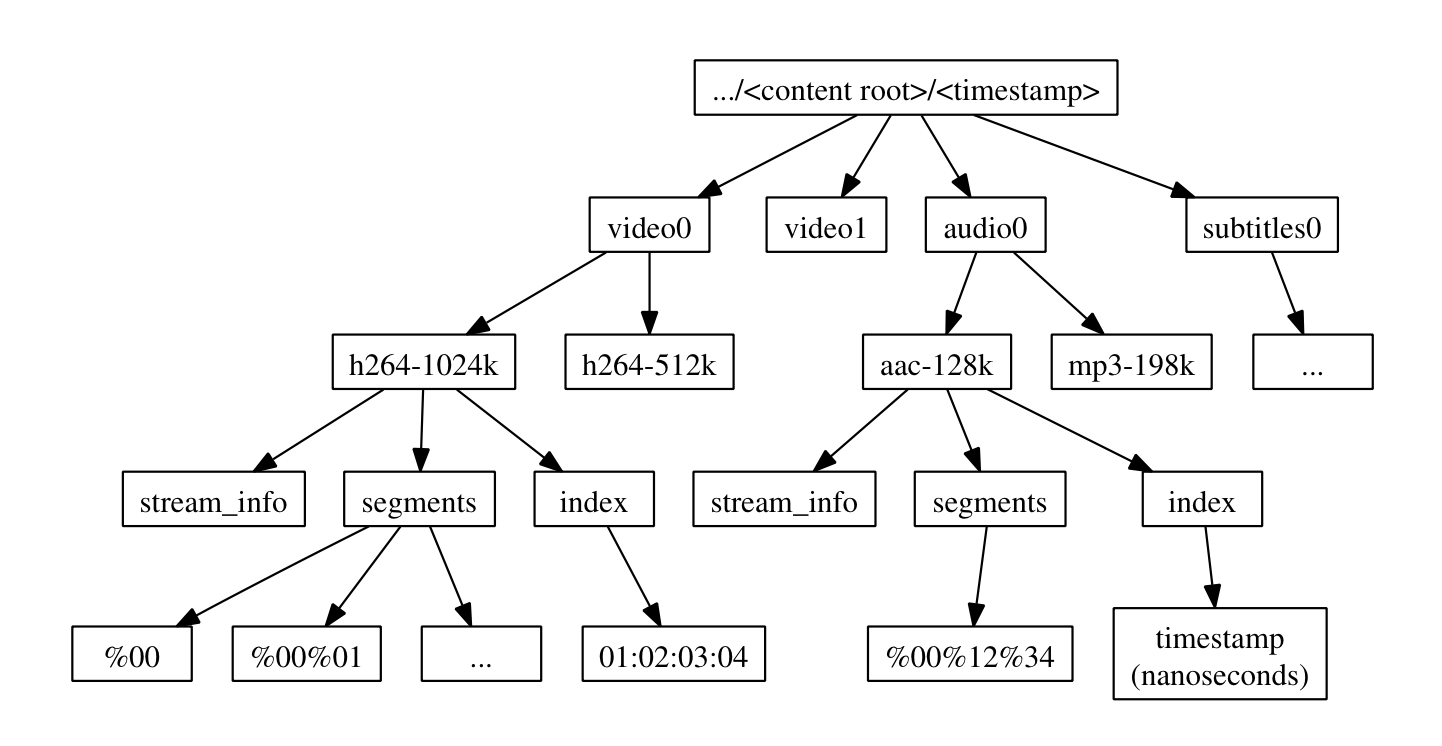
\includegraphics[scale=0.3]{ndnvideo_naming}
  % \vspace{-0.3cm}
  \caption{Prior NDNVideo Naming Space}
  \label{fig:ndnvideo_naming}
  %\vspace{-0.2cm}
\end{figure}
An similar work called NDNVideo was described in this technical report~\cite{ndnvideo}. Their aims are also to provide live and pre-recorded video streaming over NDN. They use Gstreamer to process media and Repo as the permanent storage. Producer and consumer concepts are the same, too. 

But the way how we handle framing is quite different. In the prior NDNVideo project, the video or audio stream is chopped into fixed-size segments . A mapping between time and segment number is introduced to keep the video and audio synced (Figure~\ref{fig:ndnvideo_naming}). Seeking fuction is also supported by the time-segment mapping mechanism. 

In our project, the video and audio stream is chopped into frames. One frame may contain several segments. The segmentation process is handled by Consumer / Producer API as we described above in Section~\ref{ssub:cpapi}. The application only focuses on the frame level and leaves other task to Consumer / Producer API. We think this application level framing is more like the true NDN way, which we mentioned in Section~\ref{sec:background}. Every frame has a unique name and is produced and consumed in one time. Only one frame missing won't affect other frames, thus leverages the whole impact to the playing back.

On the contrary, the fixed-size segmentation breaks the integrity of frames (ADU boundary). Only when all the packages are received correctly, the playing back progress can be guaranteed. So we think the prior NDNVideo is more like a TCP/IP way. 

The application level framing also provides the flexibility to the video consumer. For example, in NDNLive, if the previous frame can't be retrieved on time or not integrated, the consumer can just skip this bad frame to keep the video streaming. We can see from the evaluation that it won't affect the video fluency. Table~\ref{table:comparison} shows other differences such as dependencies, Gstreamer version and coding language.

\begin{table}[ht]	
	\begin{tabular}{|c|c|c|}
	\hline
	             & NDNLive \& NDNTube                                                              & NDNVideo                                                     \\ \hline 
	Dependencies & \begin{tabular}[c]{@{}c@{}}ndn-cxx / NFD\\ Consumer / Producer API\end{tabular} & \begin{tabular}[c]{@{}c@{}}CCNx / CCNR \\ pyccn\end{tabular} \\ \hline
	Gstreamer    & 1.x                                                                             & 0.1                                                          \\ \hline
	Framing      & video \& audio frames                                                           & fixed segments                                               \\ \hline
	Language     & c++                                                                             & python                                                       \\ \hline
	\end{tabular}
	\caption{Comparison with NDNVideo}
	\label{table:comparison}
\end{table}
% section comparison (end)
%%!TEX root = nextndnvideo-tr.tex
\section{evaluation} % (fold)
\label{sec:evaluation}
When some frames missing, the performance does not be affected too much. The audio will not be affected at all. For video, when the missing video frame is the key frame, it will appear one second mosaic. But if it was other type frame, the picture is fluent enough.

[I really don't know what to talk about this part... All evaluation result seems not pretty good...] -- How to measure the quantification?

% section evaluation (end)
%!TEX root = nextndnvideo-tr.tex
\section{conclusion} % (fold)
\label{sec:conclusion}
This technical report provides a detailed view on two video streaming applications: NDNlive and NDNtube.
NDNlive is capable of streaming live video captured with the camera, and NDNtube is capable of streaming video from the mp4 encoded video files. Both applications organize video and audio streams as sequences of frames, which results in a big amount of flexibility in decision making process at the consumer side of the application. Due to the increased flexibility, NDNlive consumer is able to drop the frames which have not been reassembled by the playback deadline in order to keep up with the live stream. 

NDNlive and NDNtube have different requirements for the user experience and, therefore, use different data retrieval protocols --- UDR and RDR, respectively. Both applications serve as good and relatively complete examples of using Consumer / Producer API for people who are interested in developing applications with the current implementation of the library, as well as Consumer / Producer model in general.

%\input{10-acknowledgement}

\bibliographystyle{IEEEtran}
\bibliography{references}


\end{document}
